\documentclass[10pt]{article}
\usepackage{setspace}
\usepackage{graphicx}
\usepackage{tikz}
\usepackage{float}
\usepackage{subcaption}
\usepackage{amsmath, amssymb,amsthm}
\usepackage{authblk}
\usepackage{natbib}
\usepackage{times}
\usepackage{hyperref}
\hypersetup{colorlinks=true, linkcolor=black, citecolor=black, urlcolor=blue}
\usepackage[left]{lineno}
\usepackage{algorithm}
\usepackage{algpseudocode}
\newtheorem{thm}{Theorem}[section]
\newtheorem{lem}[thm]{Lemma}
\newtheorem{prop}[thm]{Proposition}
\newtheorem{cor}{Corollary}
\newtheorem{conj}{Conjecture}[section]
% \newtheorem{as}[thm]{Assumption}
\newtheorem{defn}{Definition}[section]
\newtheorem{exmp}{Example}[section]
\newtheorem{rem}{Remark}
% \theoremstyle{definition}
\newtheorem{problem}{Problem}
% \newtheorem{definition}{Definition}
\newtheorem{example}{Example}
\usepackage[
  left =0.5in,
  right=0.5in,
  top=0.5in,
  bottom=0.5in
]{geometry}
\usepackage[percent]{overpic}
% \renewcommand\thesubfigure{\Alph{subfigure}} % A, B, C...
% \captionsetup[subfigure]{
%   labelformat=simple,
%   labelsep=none,
%   font=bf,
%   justification=raggedright,
%   singlelinecheck=false
% }

% \makeatletter
% \renewcommand\thm@headpunct{} % removes the period
% \makeatother

\newtheorem{assumption}{Assumption}
\newcommand{\assref}[1]{\hyperref[#1]{\nameref*{#1}}}

\theoremstyle{remark}
\newtheorem{note}{Note}

\newcommand{\aditya}[1]{\textcolor{blue}{\textbf{[aditya:} #1\textbf{]}}}
\newcommand{\todo}[1]{\textcolor{red}{\textbf{[NOTE:} #1\textbf{]}}}

\doublespacing

\title{\textbf{Feedback Control Analysis for Cortical Dynamics in Mice }}

\author[1]{First Author}
\author[1]{Second Author}
\author[2]{Third Author}

\affil[1]{Department of , University of Washington, Seattle, WA, USA}
\affil[2]{Department of , University of Washington, Seattle, WA, USA}

\date{}

\begin{document}
\maketitle
\linenumbers

\begin{abstract}
Dynamics of brain activity at the mesoscopic scale have been implicated in a host of perceptual, cognitive, and motor phenomena. However, establishing causal links between mesoscale dynamics and behavioral outcomes remains challenging.  In this work, we demonstrate that closed-loop optogenetic manipulation can be used to manipulate cortical activity in real time based on ongoing neural dynamics, allowing for feedback-based evaluation and manipulation of cortical dynamics.
We observe that the trial-averaged responses of a cortical region to optogenetic stimulation exhibit approximately linear, time-invariant behavior. For this setting, we design a linear output-feedback controller to modulate cortical activity using output from a cortical region to accurately track a desired reference state. We observe that this controller outperforms reference tracking, compared to an open loop stimulation across all sessions for trial-averaged responses. Moreover, we observe that trial-to-trial variability is reduced under closed loop control across all sessions, demonstrating a qualitative disturbance rejection phenomenon. Collectively, these results establish that stationary and linear averaged-dynamics can be used for modeling and controlling regional cortical activity.  
\end{abstract}


\section*{Significance Statement}
Our study introduces a closed-loop control framework for manipulating cortical activity toward a desired reference trajectory. Using wide-field calcium imaging, we extract regional cortical activity in real time and use this information to drive targeted optogenetic stimulation of neighboring areas. We demonstrate that closed-loop stimulation improves reference tracking performance in trial-averaged responses compared to open-loop stimulation. Moreover, trial-to-trial variability is significantly reduced under closed-loop control across multiple sessions and animals. Finally, we show that even during spontaneous, unstimulated activity, the underlying neuronal dynamics can be accurately approximated using linear models, supporting the feasibility of model-based closed-loop manipulation. 

\section*{Introduction}
\aditya{separately editing}
% \section{Introduction}

Neural activity at the mesoscopic scale---the coordinated fluctuations of local populations of neurons spanning multiple cortical
regions---plays a central role in sensory processing, motor control, and cognition~\citep{Churchland2012, Musall2019, Stringer2019}.
These dynamics unfold over spatial scales of hundreds of microns to millimeters and temporal scales of tens to hundreds of milliseconds,
an intermediate regime between the activity of single neurons and the global patterns observed in whole-brain imaging such as fMRI.
Understanding how mesoscale cortical dynamics give rise to behavior remains a fundamental challenge in systems neuroscience.

Wide-field calcium imaging has emerged as a powerful tool for monitoring mesoscale cortical activity in behaving
mice~\citep{Wekselblatt2016, Allen2017, Makino2017}. By combining genetically encoded calcium indicators such as GCaMP with chronic
cranial windows, wide-field imaging enables simultaneous recording of population-level fluorescence signals across the entire dorsal
cortex at frame rates sufficient to resolve behaviorally relevant dynamics~\citep{Ren2021, Ghanbari2019}. Studies using this approach
have revealed cortex-wide patterns of activation during sensorimotor tasks~\citep{Musall2019, Pinto2019}, the emergence of coordinated
cortical sequences during motor learning~\citep{Makino2017}, and the spatiotemporal structure of spontaneous cortical
activity~\citep{Mohajerani2013, Vanni2014}. Collectively, these observations suggest that the spatiotemporal dynamics of mesoscale
cortical activity carry rich information about the computational state of the brain.

A complementary line of work has sought to formalize neural population activity in terms of dynamical systems, in which the trajectory
of population-level activity evolves according to mathematically tractable rules. Seminal studies in motor cortex demonstrated that
neural population dynamics during reaching could be captured by low-dimensional, approximately linear
models~\citep{Churchland2012, Cunningham2014}. This dynamical systems perspective has since been applied across many brain areas and
behavioral contexts, revealing that complex single-neuron responses often reflect the projection of simpler population-level dynamics
onto individual cells~\citep{Vyas2020, Saxena2019}. Crucially, when viewed through population-level measurements, high-dimensional
nonlinear neural systems often admit locally low-dimensional or approximately linear representations---an observation that opens the
door to control-theoretic approaches for manipulating neural activity.

While observation of mesoscale dynamics has advanced rapidly, establishing causal links between these dynamics and behavioral outcomes
remains challenging. Optogenetics has transformed the study of neural circuits by enabling temporally precise, cell-type-specific
manipulation of neural activity~\citep{Deisseroth2011, Fenno2011}. Most optogenetic experiments employ open-loop stimulation, in which
predetermined patterns of light are delivered irrespective of the ongoing neural state. Although open-loop approaches have yielded
fundamental insights into circuit function, they are inherently limited in their ability to account for the variability and
state-dependence of neural responses~\citep{Grosenick2015}. Cortical activity fluctuates substantially from trial to trial due to
ongoing spontaneous dynamics, arousal, and behavioral state~\citep{Harris2011}, meaning that the same open-loop stimulus can produce
widely varying neural and behavioral effects depending on the brain state at the time of stimulation.

Closed-loop paradigms, in which stimulation is continuously adjusted based on real-time measurements of neural activity, offer a
principled framework for overcoming these limitations. From a control-theoretic perspective, feedback enables a system to compensate
for unmodeled disturbances and maintain a desired output despite variability in the underlying activity state or
dynamics~\citep{Astrom1995}. In the context of neural manipulation, closing the loop provides two key advantages: it allows
stimulation to adapt to the current brain state, improving the precision of neural modulation; and it enables the experimenter to
drive neural activity toward specific target trajectories, creating opportunities for causal tests that are not possible with
open-loop stimulation alone~\citep{OShea2018}.

Several groups have demonstrated the feasibility and utility of closed-loop optogenetic control at the level of single neurons and
local field potentials. \citet{Newman2015} introduced the ``optoclamp,'' a proportional--integral (PI) controller that locked the
firing rate of individual neurons to stationary targets in cultured networks and in the anesthetized rat thalamus.
\citet{Bolus2018} developed model-based design strategies for dynamic closed-loop optogenetic neural control in vivo, and subsequently
demonstrated state-space optimal feedback control of single-neuron firing rates in awake, head-fixed mice using linear-quadratic
optimal control~\citep{Bolus2021}. At the network level, closed-loop optogenetic stimulation has been used to modulate oscillatory
dynamics in brain slices and in non-human primates~\citep{Nicholson2018, Cagnan2023}. \citet{Clancy2014} showed that closed-loop
optogenetic feedback could train mice to modulate neural activity in motor cortex, establishing that neural circuits can be shaped
through activity-dependent stimulation. A comprehensive review by \citet{Grosenick2015} outlined the theoretical and practical
foundations for closed-loop optogenetic control, emphasizing its potential for causal circuit dissection.

Despite these advances, most prior closed-loop optogenetic studies have operated at the level of single neurons or local field
potentials, using electrophysiological recordings as the feedback signal. The application of closed-loop control to mesoscale cortical
population dynamics---using wide-field calcium imaging as the readout---remains largely unexplored. This gap is significant because
mesoscale dynamics reflect the integrated activity of large neuronal populations and are directly relevant to the kinds of distributed
cortical computations that underlie perception and behavior. Moreover, recent technical developments have made it possible to perform
simultaneous wide-field calcium imaging and spatially targeted optogenetic stimulation across the dorsal cortex of awake
mice~\citep{Matveev2024}, providing the experimental infrastructure needed for real-time, mesoscale closed-loop control.

Here, we demonstrate a closed-loop optogenetic control framework for regulating mesoscale cortical population activity in head-fixed
mice. Using wide-field calcium imaging, we extract a real-time readout of regional cortical activity ($\Delta F/F$) and use this
signal to drive a proportional--integral (PI) feedback controller that modulates targeted optogenetic stimulation of a neighboring
cortical region. We first characterize the input--output relationship between optogenetic stimulation and trial-averaged cortical
responses, showing that this relationship is well approximated by a linear mapping---a finding that enables principled, model-based
controller design. We then implement a PI controller with feedforward compensation and demonstrate that closed-loop stimulation
improves reference tracking accuracy and reduces trial-to-trial variability compared to open-loop stimulation across multiple
experimental sessions and animals. The reduction in variability is interpreted as an active disturbance rejection phenomenon,
wherein feedback suppresses the influence of spontaneous cortical fluctuations on the driven response. Collectively, these results
establish that stationary, approximately linear trial-averaged dynamics can be exploited for modeling and controlling regional
cortical activity, and demonstrate the potential of feedback-based perturbation paradigms for causally investigating cortical
population dynamics.
   
% %%%%%%%%%%%%%%%%%%%%%%%%%%%%%%%%%%%%%%%%%%%%%%%%%%%%%%%%%%%%
\section*{Results}
% %%%%%%%%%%%%%%%%%%%%%%%%%%%%%%%%%%%%%%%%%%%%%%%%%%%%%%%%%%%%

We developed a real-time closed-loop optogenetic system to regulate population activity within a targeted cortical region, monitored using wide-field calcium imaging. Trial-averaged cortical responses to optogenetic stimulation obeyed a stationary linear input--output map, providing the empirical foundation for controller design.

% ------------------------------------------------------------
\subsection*{Experimental setup and closed-loop control architecture}
% ------------------------------------------------------------ 
The closed-loop experiments were performed in head-fixed transgenic GCaMP and opsin-expressing mice in a behavioral chamber \citep{Matveev2024}. The front limbs of the mice rested on a freely moving wheel, and a blank screen was present in front of the mouse.
Neural activity was recorded at 35\,Hz using wide-field calcium imaging (Fig.~\ref{fig:figure1}A), and spatially resolved optogenetic stimulation was applied to a targeted cortical region neighboring the $\Delta F/F$ output zone as depicted in Fig.~\ref{fig:figure1}B. The stimulation region was picked to be close to the output kernel (Fig.~\ref{fig:figure1}C) so as to directly inhibit the region's activity.
We then designed a hardware and software architecture for signal processing and fast closed-loop control of this mesoscale activity (Fig.~\ref{fig:figure1}D). The software layer handled the mathematical framework required for computing control signal through feedback.
We designed a proportional--integral (PI) feedback controller with open-loop compensation to drive cortical activity toward the reference $\Delta F/F$ value(Fig.~\ref{fig:figure1}E).
The open-loop component provided the nominal stimulus required to reach a reference state based on the calibrated controller gains, while the PI feedback component added real-time error correction to compensate for bias due to inaccurate open loop gains, residual nonlinearities, and spontaneous trial-to-trial fluctuations.
The control system as depicted in Fig.~\ref{fig:figure1}E, treats the kernel averaged wide-field measurements as outputs, the controller uses the error between output and reference signal to compute an optogenetic stimulus input to the plant, subject to a processing and physiological delay that closes the loop (Fig.~\ref{fig:figure1}F). The system has an inherent maximum latency of 47\,ms, computed as the time between signal arrival at the cortical level and application of the laser.

\begin{figure}[h]
    \centering
    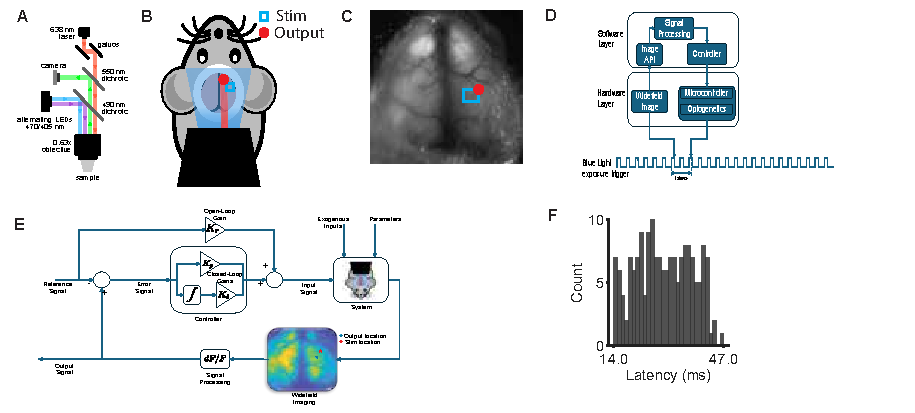
\includegraphics[width = \linewidth]{images/Figure1.pdf}
    \caption{Experimental setup and closed-loop control architecture.\\
    \small{
    \textbf{A:} Schematic of the widefield microscope optical path. Blue (470\,nm) and violet (405\,nm) LEDs illuminate the dorsal cortex; emitted green photons are collected by the camera via two dichroics. A red (638\,nm) galvanometer-steered laser passes through both dichroics to deliver spatially targeted optogenetic stimulation.\\
    \textbf{B:} Dorsal cortex schematic showing the spatial relationship between the optogenetic stimulation target (red) and the $\Delta F/F$ output region (blue box).\\
    \textbf{C:} Representative widefield frame showing the stimulation spot (red) and the spatial kernel used as the closed-loop feedback output (blue box).\\
    \textbf{D:} Signal-flow diagram of the closed-loop pipeline. A hardware trigger initiates frame acquisition; the image API streams frames to the control server, which computes $\Delta F/F$ and evaluates the controller; the resulting command drives the optogenetic stimulator via a microcontroller.\\
    \textbf{E:} Block diagram of the closed-loop control architecture. The spatial-kernel $\Delta F/F$ average provides the output $y_t$; the PI controller computes a corrective input from the tracking error and sums it with the feedforward term; the combined signal drives the laser, subject to an end-to-end latency of 80\,ms.\\
    \textbf{F:} Distribution of measured end-to-end control-loop latencies across all sessions (3 mice, 13 sessions). Latency is defined as the time from camera trigger to laser activation command, encompassing image transfer, $\Delta F/F$ computation, and digital-to-analog conversion.
    }}
    \label{fig:figure1}
\end{figure}

% ------------------------------------------------------------
\subsection*{Trial-averaged cortical dynamics are approximated by a linear system}
% ------------------------------------------------------------
Trial-averaged cortical responses followed a linear input--output map for impulse based stimulation, and a linear dynamical system closely approximated impulse and step responses for cortical stimulation using optogenetics. 
We delivered optogenetic impulse inputs at discrete amplitudes between 0--1.8\,mW powers, randomly interleaved across trials for each session. The Fig.~\ref{fig:figure2}A, shows the trial averages impulse response for one of the experiment sessions, which is used to characterize settling time($\sim200$ms) for impulse response.
We found that the mean of the distribution of total inhibition energy(see Methods) per trial, had a monotonic relationship with stimulation amplitudes, therefore it could be approximated with a linear relationship across the three sessions (Fig.~\ref{fig:figure2}B; $R^{2} = 0.99, 0.51, 0.94$; slope $= -0.36, -0.57, -0.58$). This linear relationship between stimulation amplitude and inhibition energy supports the design of an open-loop controller calibrated from impulse response data that relies on monotonicity of the input output relationship~\citep{astrom1995pid}.

\begin{figure}
    \centering
    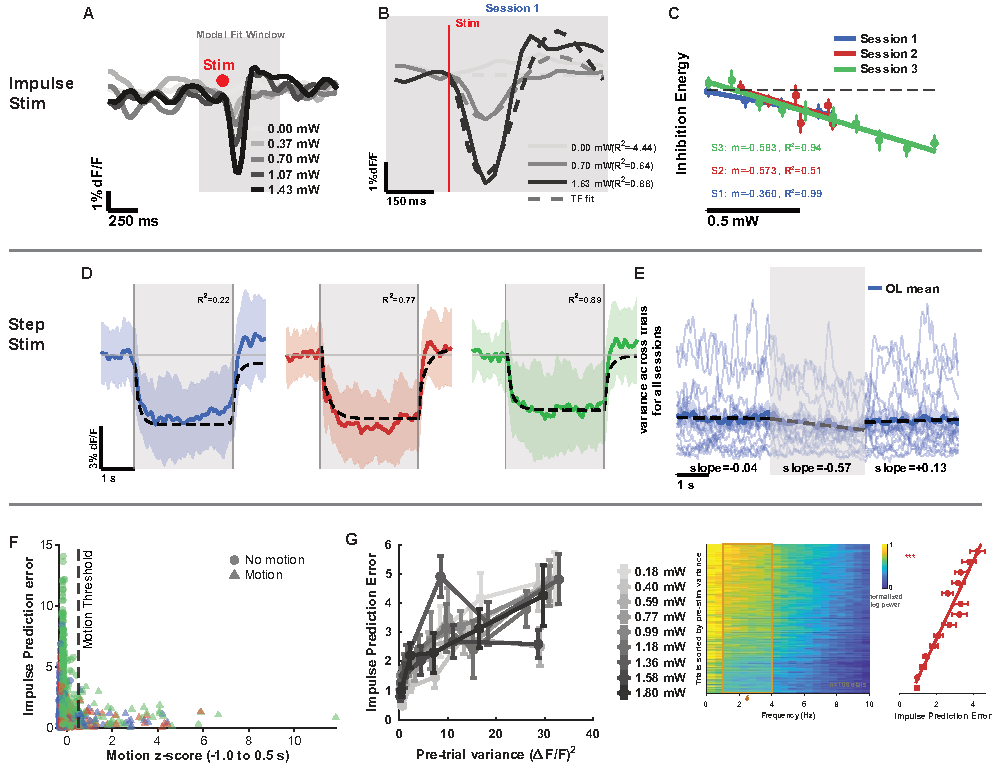
\includegraphics[width = \linewidth]{images/Figure2_extra.pdf}
    \caption{Input-output characterization of local cortical dynamics.\\
    \small{
    \textbf{A:} Trial-averaged $\Delta F/F$ impulse responses across five stimulation amplitudes (0--2.7\,V; $\sim$90 trials per amplitude). Traces are aligned to stimulation onset (red line); shading shows $\pm$1\,SD across trials. Amplitude was randomly sampled on each trial.\\
    \textbf{B:} Inhibition energy denoting the total suppression for 0-200ms versus stimulation amplitudes for three sessions. Points show mean $\pm$ SD across trials ($\sim$50 trials per amplitude); lines show the fitted linear input-output relationship (see Methods). $R^{2} = 0.94, 0.51, 0.99$ across three sessions.\\
    \textbf{C:} Prediction of trial-averaged traces of three representative impulse responses. The bold traces show the trial-averaged response and the dashed responses show LTI system fit to the trial averaged data($N = 90 $trials).
    \textbf{D:} Prediction of trial-averaged traces of three representative step responses. The bold traces show the trial-averaged response and the dashed responses show LTI system fit to the trial averaged data($N = 50 $trials).
    \textbf{E:} Traces showing variance across trials for an experiment session. We show variance traces for 13 session across stimulation window(gray) of three seconds, along with 3 second pre and post stim windows. The bold trace shows average of all variance traces. The dashed lines show the linear approximation of the average variance trace, the slope of this line is shown for the pre, during, and post sti windows.}}
    \label{fig:figure2}
\end{figure}

Step inputs applied over 3-second trial windows produced trial-averaged trajectories that were closely approximated by a LTI system. We fit LTI systems to trial-averaged, step response data from three different sessions as shown in Fig.~\ref{fig:figure2}D. The LTI system was fit to learn step response of a low dimensional transfer function 
consistent with marginally stable oscillatory dynamics in biologically bounded cortical circuits. 
Open-loop stimulation modestly reduced across-trial variance during stimulation (post-onset slope $-0.57 \pm 0.24$\,($\Delta F/F$)$^2$/s, vs.\ near-zero pre-onset slope $-0.04 \pm 0.14$, $n=13$ sessions); closed-loop feedback produced a further and more consistent reduction. Under open-loop step stimulation, trial-to-trial variance did not change around stimulus onset (Fig.~\ref{fig:figure2}C), indicating that optogenetic input did not destabilize the system.
Session-to-session offset bias in the step response informed inclusion of the integral term in the PI controller (see Materials and Methods).
Batch-mean $\Delta F/F$ variance during spontaneous activity decreased monotonically with trial count, stabilizing beyond approximately 50 trials per session (Fig.~\ref{fig:S1}), consistent with the trial-averaging assumption (see Materials and Methods). \todo{Also verify that the batch mean itself stabilizes across batch sizes — variance convergence (CLT) holds for any finite-variance process including drifting ones, and does not alone establish zero-mean disturbances.}
Convergence rates differed across sessions recorded from the same region, consistent with session-to-session differences in brain state.

% ------------------------------------------------------------
\subsection*{Closed-loop control improves reference tracking accuracy}
% ------------------------------------------------------------

Across sessions in \todo{INCONSISTENCY: this says ``two mice'' but Fig.~3 caption says ``3 mice, 13 sessions'' and Fig.~1F caption also says ``3 mice, 13 sessions''. Determine the correct mouse count (AL\_0033 + AL\_0039 = 2 mice, but total sessions = 13 spans additional animals?) and apply consistently throughout.} two mice with confirmed opsin expression, closed-loop feedback consistently improved tracking of $y_{\mathrm{ref}} = -5\%\,\Delta F/F$ relative to open-loop stimulation (Fig.~\ref{fig:figure3}A--D). 
Under open-loop conditions, the feedforward term produced cortical responses that systematically deviated from the reference, reflecting the inability of a fixed input to compensate for ongoing spontaneous fluctuations or inaccuracies in the estimated gain $K_{r}$.
Under closed-loop control, the proportional term corrected instantaneous deviations while the integral term accumulated and eliminated persistent offset, yielding substantially improved alignment with $y_{\mathrm{ref}}$ at the single-trial level (Fig.~\ref{fig:figure3}A).


\begin{figure}
    \centering
    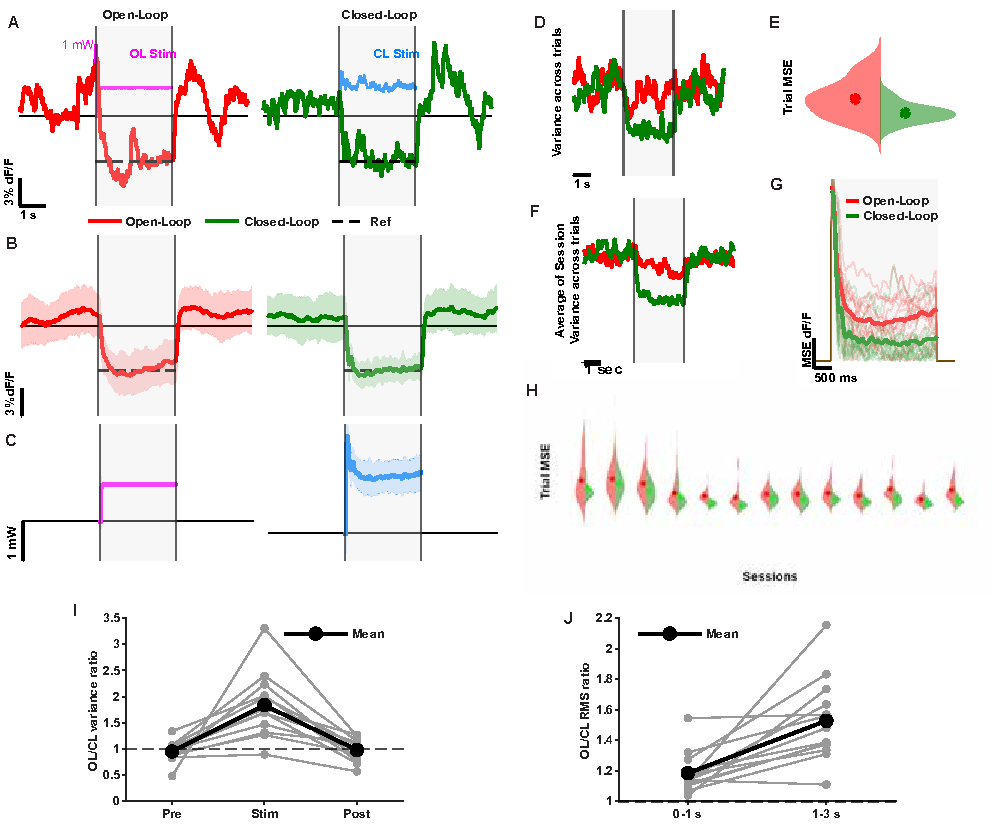
\includegraphics[width = \linewidth]{images/Figure3_extra.pdf}
    \caption{Closed-loop versus open-loop cortical activity control (2 mice, 13 sessions).\\
    \small{
    \textbf{A:} Single-trial example of open-loop (red) and closed-loop (green) $\Delta F/F$ responses. Gray shading marks the 3\,s stimulation window; dashed line indicates the target $-5\%\,\Delta F/F$. Bottom traces show the corresponding optogenetic input signals.\\
    \textbf{B:} Trial-averaged $\Delta F/F$ responses under open-loop (red) and closed-loop (green) control for a representative session. Bold lines show the trial mean; thin lines show individual trials.\\
    \textbf{C:} Trial-averaged optogenetic input signals for open-loop (pink) and closed-loop (blue) conditions. Bold lines show the mean input; thin lines show individual trials.\\
    \textbf{D:} Cross-trial variance of $\Delta F/F$ as a function of time for open-loop and closed-loop conditions, for a representative session. Gray shading marks the stimulation window.\\
    \textbf{E:} Distribution of per-trial tracking MSE (mean squared error over the 3\,s stimulation window) for open-loop and closed-loop conditions, shown as violin plots. Points indicate individual trials.\\
    \textbf{F:} Cross-trial variance during the stimulation window, averaged across all 13 sessions, for open-loop and closed-loop conditions.\\
    \textbf{G:} Per-trial MSE distributions pooled across all 13 sessions, shown as violin plots.\\
    \textbf{H:} Mean absolute tracking error per unit time as a function of time within the trial, averaged across all sessions (bold) with individual session traces (thin lines).\\
    \textbf{I:} Ratio of variance across trials for OL and CL trials for each session, for pre-stim window(stim-start $- 3$sec to stim), stim window and post stim (stim-end to stim-end $+3$ seconds) window. The gray lines depict individual sessions and bold line represents mean of all sessions.\\
    \textbf{J:} Controller disturbance rejection effect shown by splitting trial into $0-1$sec and $1-3$sec regimes depicting setting time and stable activity regimes, the y-axis show ratio of OL and CL tracking error RMS for each experiment session. The gray lines depict individual sessions and bold line represents mean of all sessions.
    }}
    \label{fig:figure3}
\end{figure}

Trial-averaged responses confirmed that closed-loop activity followed the reference closely throughout the stimulation window, whereas open-loop responses exhibited systematic positive bias (Fig.~\ref{fig:figure3}B).
The difference in average input responses between conditions (Fig.~\ref{fig:figure3}C) reflects the additional corrective signal contributed by real-time feedback. 
Per-trial tracking costs shifted toward lower values and showed reduced spread under closed-loop control (Fig.~\ref{fig:figure3}E), indicating both improved mean performance and enhanced reliability of neural modulation across trials. \todo{Re-compute per-trial MSE over t = +1 s to +3 s post-laser onset; update figures and text once recomputed (see MEETINGS.md 2026-05-08).}
These improvements held across all recorded sessions (Fig.~\ref{fig:figure3}G) and required small controller gains. For the session shown in Fig~\ref{fig:figure3}A-E we used the gains, $K_{r} = \mathbf{0.1}, K_{p} = \mathbf{0.07} \& K_{i} = \mathbf{0.1}$, suggesting that the approximately linear, stationary input--output structure identified empirically was sufficient to support stable PI feedback.

% ------------------------------------------------------------
\subsection*{Brain states affects predictability}
% ------------------------------------------------------------

\todo{SECTION INCOMPLETE — write the pre-stimulus brain state paragraph here. Key result (FINDINGS.md, prestim\_variance.m): OL regression slope of pre-stim variance vs.\ per-trial MSE is positive (higher pre-stim variance $\to$ higher error); CL slope is near-flat, indicating feedback decouples performance from initial brain state. Add K2 figure reference. Also implement Curto \& Issa-style trial-sorting figure: split trials by $\sim$1\,s pre-stim variance (synced vs.\ desynced); sort within groups by $|\Delta F/F|$ at $t=0$; display heatmaps for OL and CL. Verify authorship: Curto, Bhatt \& Issa (2009) before citing. Consider 500\,ms or sliding window instead of 1\,s (may conflate state transitions, per MEETINGS 2026-05-11).}

% ------------------------------------------------------------
\subsection*{Closed-loop control reduces trial-to-trial variability}
% ------------------------------------------------------------
In addition to improving mean tracking accuracy, closed-loop feedback substantially reduced trial-to-trial variability in cortical activity during the stimulation window (Fig.~\ref{fig:figure3}D--F). 
This result follows from the structure of the PI controller: individual trial trajectories are perturbations of the nominal averaged response driven by zero-mean neural disturbances and trial-to-trial brain-state fluctuations, and the controller actively steers each trial back toward the reference, compressing the cross-trial distribution of responses.

\todo{INCONSISTENT WITH FINDINGS: ``remained largely unchanged'' contradicts the variance claim fix needed at the sentence above (post-onset OL slope $= -0.57 \pm 0.24$ is not ``unchanged''). Once the variance sentence in the previous section is rewritten, update this sentence to match — likely: ``Under open-loop stimulation, variance modestly decreased relative to the pre-stimulation baseline\ldots''} During open-loop stimulation, response variance remained largely unchanged relative to the pre-stimulation baseline, reflecting the inability of the fixed feedforward term to counteract spontaneous fluctuations. Under closed-loop control, variance decreased substantially during the stimulation window, consistent with active disturbance rejection. This reduction persisted across sessions, as confirmed by pooled within-session variance traces (Fig.~\ref{fig:figure3}D--F) and by the cross-session distribution of per-trial MSE (Fig.~\ref{fig:figure3}G).

The validity of these results depends on the trial-averaging assumption holding across the session. The empirical variance convergence in Fig.~\ref{fig:S1} supports this assumption over the 100-trial validation period. 
Performance varied across animals and sessions, likely reflecting residual non-stationarity in arousal and behavioral state, differences in opsin expression, and session-to-session variation in the spatial overlap between stimulation and output regions.
Despite this variability, directional improvements in both tracking accuracy and trial-to-trial variance were consistent across all experiments.


We observed that motion affected trials 
\todo{PLACEHOLDER — Curto \& Issa-style trial-sorting figure (see MEETINGS.md 2026-05-11). Split trials into synchronized (high pre-stim variance, $\sim$1\,s window) vs.\ desynchronized (low pre-stim variance). Within each group, sort trials by absolute fluorescence at $t = 0$. Display $\Delta F/F$ heatmaps for CL and OL conditions. Verify authorship before citing: Curto, Bhatt, Issa (2009). Note: 1\,s pre-stim window may conflate state transitions — consider 500\,ms or sliding window.}

% ------------------------------------------------------------
\subsection*{Disturbance attribution: spectral and motion analysis}
% ------------------------------------------------------------
\todo{PLACEHOLDER — Confirm absolute power spectra (ΔF/F$^2$/Hz) complete; finalize narrative framing (motion + frequency → trial outcome). Determine what fraction of high-error CL trials are attributable to 2--4\,Hz spontaneous fluctuations vs.\ motion. Add motion vs.\ MSE (CL vs.\ OL, cross-session) scatter panel and good/bad trial spectral examples to manuscript (see MEETINGS.md 2026-05-11).}

% ------------------------------------------------------------
\subsection*{Contralateral cortex predicts ipsilateral activity}
% ------------------------------------------------------------
\todo{PLACEHOLDER — Three-layer contralateral-prediction model figure (see MEETINGS.md 2026-05-11). Pink: predict ipsilateral ROI from contralateral pixels in spontaneous (no-opto) data. Orange: add average OL impulse response on top. Red: add per-trial laser sequence via TF model; validate against CL traces. Add motion energy as co-predictor. If red model validates: compute post-hoc optimal laser sequence for representative trials, quantify gap vs.\ actual controller, frame as MPC motivation.}

% ------------------------------------------------------------
\subsection*{Feedforward and preview control}
% ------------------------------------------------------------
\todo{PLACEHOLDER — Feedforward (sine-wave) and preview control results (deferred since 2026-04-27; see PAPER.md). Add plots for variable sine-wave reference. Classify feedforward vs.\ preview control. Compare against naive CL baseline. Requires new section in manuscript with literature context.}

\section*{Discussion}

In this study, we demonstrate that closed-loop optogenetic stimulation driven by real-time wide-field calcium imaging can regulate mesoscale cortical population activity more reliably than open-loop stimulation. By dynamically adjusting optogenetic input using the PI feedback controller (Equation~\ref{eq:controller}), cortical population activity was driven toward a predefined reference trajectory across experimental sessions and animals. Closed-loop feedback improved tracking
accuracy, reduced mean-squared error as measured by $\hat{J}(K)$ (Equation~\ref{eq:emp_cost}), and reduced trial-to-trial variability. Collectively, these results demonstrate that the approximately linear, stationary structure of trial-averaged cortical dynamics captured by Assumption~\ref{sec:assumption1} can be exploited to design simple but effective output-feedback controllers for mesoscale neural regulation.

\subsection*{Linear approximation of mesoscale cortical dynamics enables controller design}

A central result enabling our framework was the empirical demonstration that trial-averaged cortical responses to optogenetic stimulation are well approximated by a linear input--output map. The theoretical basis for this is the LPV model (Equations~\ref{eq:lpv_state}--\ref{eq:lpv_output}), in which the parameter $\rho$ varies across trials due to spontaneous fluctuations in arousal, behavioral state, and network dynamics. Under \textbf{trial-averaging} Assumption~\ref{sec:assumption1}, taking expectations over $\rho$ and $d$ yields the nominal LTI system $(\bar{A}, \bar{B}, C) = (\mathbb{E}_\rho[A(\rho)],\, \mathbb{E}_\rho[B(\rho)],\, C)$, whose input--output behavior corresponds to the observed trial-averaged dynamics. This averaging framework explains why linearity is observed in expectation even when individual trials reflect the richer dynamics of
Equations~\eqref{eq:nl_state}--\eqref{eq:nl_output}: the contributions of $\rho_t$ and $d_t$ cancel in the mean when drawn from stationary, zero-mean distributions. 

This finding is consistent with a broader literature demonstrating that complex nonlinear neural population dynamics often admit locally low-dimensional or approximately linear representations when viewed through population-level measurements~\citep{Churchland2012, Cunningham2014, Stringer2019}. Identifying this structure at the mesoscale, using trial averaging to suppress the influence of spontaneous variability, provides a tractable basis for controller design without requiring explicit system identification. Crucially, inaccuracies in the feedforward gain $K_r$ (Equation~\ref{eq:Kr}) arising from session-to-session differences in opsin expression, spatial alignment, external stimulus, or brain state are compensated online by the integral term of Equation~\eqref{eq:controller}, making the approach robust to moderate model mismatch.

The trial-averaged step responses did not definitively converge to a steady state within the 3-second trial window, varying across sessions in overshoot and offset. But the traces remain within an invariant set around the activity mean. We interpret this as a property of marginally stable dynamics of biologically bounded cortical circuits, in which activity remains close to a stationary mean rather than decaying to a fixed equilibrium~\citep{hespanha2018linear}, rather than as evidence against linearity. 

%Consistent with the brain-state analysis in the Results, trials recorded during desynchronized, low-power epochs~\citep{Harris2011} exhibited more predictable and monotonic input--output responses, whereas synchronized states yielded less reliable behavior. These observations highlight the importance of monitoring arousal state in future closed-loop experiments and suggest that adaptive mechanisms for detecting and responding to brain-state transitions could substantially improve controller robustness.

\subsection*{Disturbance rejection underlies variability reduction}

The reduction in trial-to-trial variability observed under closed-loop stimulation has a natural interpretation within the LPV framework (Equations~\ref{eq:lpv_state}--\ref{eq:lpv_output}). Under Assumption~\ref{sec:assumption1}, individual
trial responses are perturbations of the nominal trajectory $\bar{\Sigma}_{\bar{x}_0}$ driven by the disturbance $d_t$
and parameter variation $\rho_t - \bar{\rho}$. These perturbations are zero-mean in expectation but nonzero on
individual trials, and they constitute the primary source of cross-trial variance under open-loop conditions. The PI
controller (Equation~\ref{eq:controller}) suppresses these deviations through two complementary mechanisms: the
proportional term $K_p(y_{\mathrm{ref}} - y_t)$ provides immediate timestep-level correction, while the integral term
accumulates error across time to eliminate persistent offsets arising from bias in $K_r$ or slow drift in the latent
state. Together, these terms implement active disturbance rejection within the augmented closed-loop system
(Equations~\ref{eq:aug_state}--\ref{eq:aug_output}).

From a control-theoretic standpoint, this mechanism does not require knowledge of the disturbance structure---only that
the input--output relationship is approximately monotonic in expectation~\citep{Astrom1995}, which the impulse response
characterization confirmed. The convergence $\hat{J}(K) \to J(K)$ guaranteed by Trial-averaging Assumption~\ref{sec:assumption1}
further implies that variance reduction will be most reliable when brain state is approximately stationary across the
session, consistent with the empirical observations and with the variance convergence in Figure~\ref{fig:variance_batch}.

\subsection*{Relation to prior closed-loop neural control work}

These results contribute to a growing literature demonstrating the feasibility of closed-loop optogenetic control for manipulating neural circuit dynamics. \citep{Newman2015} introduced a PI ``optoclamp'' that locked single-neuron firing rates to stationary targets in cultured networks and the anesthetized rat thalamus, establishing the feasibility of the PI control structure used here. \citep{bolus2021state} demonstrated state-space optimal feedback control of single-neuron firing rates in awake mice using linear-quadratic (LQ) design strategies requiring explicit system identification~\citep{van2012subspace} and disturbance identification. Our approach differs in that the underlying system is not identified step-by-step; instead, Assumption~\ref{sec:assumption1} is exploited to bypass full identification, and the integral term of Equation~\eqref{eq:controller} compensates for model inaccuracies online. This makes the framework accessible in settings where the non-stationarity and parameter dependence of the cortical response render classical identification methods infeasible within the given experimental time-frame.

At the network level, closed-loop optogenetic stimulation has been used to modulate oscillatory dynamics in brain slices and non-human primates~\citep{Zaaimi2022}, and \citet{Clancy2014} demonstrated that activity-dependent feedback could shape motor cortex dynamics in behaving mice. Our work differs from this literature on the mesoscale, by using population-level $\Delta F/F$ as the feedback signal rather than electro-physiological recordings. Unlike many brain--computer interface (BCI) paradigms that regulate neural activity indirectly via behavioral outputs, the present framework directly targets cortical population dynamics, enabling closed-loop manipulation of the trajectories most relevant to distributed cortical computation~\citep{Grosenick2015, OShea2018}.


\subsection*{Sources of variability and experimental limitations}

Several factors shaped and limited closed-loop performance. First, the empirical cost estimate $\hat{J}(K)$
(Equation~\ref{eq:emp_cost}) approximates $J(K)$ (Equation~\ref{eq:expected_cost}) with the regret $R(N, K)$
(Equation~\ref{eq:regret}), which decreases only if trials are independently drawn from a stationary brain-state
distribution. In practice, if cortical state drifts during evaluation of one candidate controller and shifts during
evaluation of another, the resulting estimates of $\hat{J}(K)$ can be biased in opposite directions, inflating the
apparent performance difference between controllers. This risk was mitigated by randomly interleaving open-loop and
closed-loop trials, but cannot be eliminated entirely given the non-stationarity of awake, behaving animals. Episodes
of sustained locomotion or drowsiness represent the most likely sources of such bias, as they correspond to brain-state
regimes in which Assumption~\ref{sec:assumption1} is least likely to hold.

Second, the actuator saturation enforced at 36\,mW (5\,V; see Section~\ref{sec:pi_controller}) constrained the
controller's ability to track $y_{\mathrm{ref}}$ during epochs of high spontaneous activity that demanded large
corrective inputs. Future implementations could benefit from adaptive reference trajectories that adjust
$y_{\mathrm{ref}}$ based on the estimated current cortical state, or from optogenetic actuators with a wider dynamic
range.

Third, the 80\,ms control-loop latency (Figure~\ref{fig:system}A) spans approximately three 35\,Hz timesteps and
limits the bandwidth of disturbance rejection for fast spontaneous fluctuations. Optimization of onboard computation
and hardware communication could reduce this latency and extend the effective control bandwidth, particularly for
rejecting high-frequency cortical oscillations.

\subsection*{Future directions}

We proposed a low-level control algorithm for regulating local cortical activity. The controller was a good regulator of local dynamics. The implications of this work are that such controllers can be used to drive the dynamics precisely to a specific target trajectory. The direct implication of this work is that we can extend this work to be paired with a model-predictive control, where a this internal PI control can reliably track the high level dynamics. We propose that this controller can be paired with a latent dynamics prediction setup, to reliably track behavior inducing activity. 

% The model-free zeroth-order gain optimization (Algorithm~\ref{alg:zeroth_order}) demonstrated that a well-performing
% gain region is reachable within a physiologically feasible number of trials. This algorithm can be further optimized by using approximate gradient which can be computed from data, to exploit 'momentum' update direction. Using offline model information can further aid in approximating update direction.  
% Pairing the present framework with
% model predictive control (MPC) or online adaptive strategies that estimate the latent state $x_t$ in real time would
% enable tracking of time-varying reference trajectories, explicit handling of actuator constraints within a receding
% horizon, and principled adaptation to brain-state transitions that currently violate Assumption~\ref{sec:assumption1}.

More broadly, closed-loop regulation of mesoscale cortical activity opens several experimental and translational
avenues. Feedback-based perturbation paradigms can be used to test causal dynamical systems hypotheses about cortical
computation---for example, by driving activity along specific reference trajectories and measuring downstream behavioral
or circuit-level consequences~\citep{OShea2018}. The disturbance rejection capability of the PI
controller~\eqref{eq:controller} may also prove useful for stabilizing pathological patterns of cortical dynamics, such
as the abnormal synchrony associated with epilepsy or neuropsychiatric disorders. Combining mesoscale closed-loop
control with simultaneous electrophysiology could further bridge the gap between the population-level feedback signals
used here and the single-neuron mechanisms that give rise to them.

The existing PI controller can also be further enhanced by implementing a parameter dependent multi-modal design. The existing controller relies heavily on the trial-averaging assumption, and assumes that brain states are not being identified. If the stimulation has significant difference in effect with respect to brain states, then a gain scheduled controller can be employed such that the controller switches to states specific gains.
Another avenue for improvement of regulation would be consideration of a data-driven model for controller design where, using data from a finite horizon in the past, a controller strategy is devised so that the 

% %%%%%%%%%%%%%%%%%%%%%%%%%%%%%%%%%%%%%%%%%%%%%%%%%%%%%%%%%%%%
\section*{Materials and Methods}
% %%%%%%%%%%%%%%%%%%%%%%%%%%%%%%%%%%%%%%%%%%%%%%%%%%%%%%%%%%%%

% ------------------------------------------------------------
\subsection*{Animals}
% ------------------------------------------------------------

We conducted all experiments in adult transgenic mice (8--20 weeks)
expressing either GCaMP6s or GCaMP8s in excitatory cortical neurons
under the CaMKII promoter. To enable simultaneous wide-field calcium
imaging and optogenetic perturbation, animals received a retro-orbital
injection of a PHP-eB serotype adeno-associated viral (AAV) vector
carrying a DLX2.0-driven Chrimson construct, which restricts opsin
expression to inhibitory interneurons and thereby enables focal cortical
suppression through inhibitory activation with minimal spectral
cross-talk with GCaMP imaging. This dual-expression configuration
permitted mesoscale calcium measurement via GCaMP fluorescence and
spatially localized, optogenetically driven suppression within the same
field of view. All procedures were approved by the Institutional Animal
Care and Use Committee (IACUC) at the University of Washington and were
conducted in accordance with NIH guidelines for the care and use of
laboratory animals.

% ------------------------------------------------------------
\subsection*{Surgical preparation and habituation}
% ------------------------------------------------------------

We implanted a chronic trans-cranial window over the dorsal cortex to
provide stable, long-term optical access to the entire dorsal cortical
surface in awake animals, following procedures described previously
\citep{Matveev2024}. Briefly, we removed the scalp and periosteum and
applied thin layers of UV-cured optical glue to the exposed skull
surface inside a 3D-printed recording chamber secured with dental
cement, maintaining transparency over the imaging field of view. We
attached a custom head-plate to allow reproducible head-fixation across
sessions. Animals were allowed at least one week of recovery before any
experimental handling.

% ------------------------------------------------------------
\subsection*{Wide-field calcium imaging}
% ------------------------------------------------------------

We recorded neural activity using a custom single-photon mesoscopic
fluorescence microscope with excitation and emission filters matched to
the GCaMP spectrum. We acquired images at 70\,Hz with a
$9.7\,\mathrm{mm} \times 9.7\,\mathrm{mm}$ field of view, providing
mesoscale coverage of the entire dorsal cortical surface at a pixel
resolution sufficient to resolve regional population dynamics. We
collected frames using alternating blue (470\,nm) and violet (405\,nm)
illumination at 35\,Hz per channel; the violet channel captures
hemodynamic absorbance and tissue autofluorescence for correction
purposes and was not used for real-time computation. We maintained light
power below levels known to elicit phototoxicity or direct
photostimulation of Chrimson.

For offline analysis, we preprocessed imaging data using a standard
pipeline including rigid motion correction, reflectance normalization,
and computation of $\Delta F/F$. We registered frames to a common
anatomical reference atlas and temporally aligned stimulation event
timestamps to the imaging data stream for trial-level analysis. Full
hardware specifications, surgical details, and viral constructs are
described in \citet{Matveev2024}.

% ------------------------------------------------------------
\subsection*{Optogenetic stimulation}
% ------------------------------------------------------------

We delivered optogenetic stimulation concurrently with imaging via a
secondary, spatially targeted illumination pathway tuned to the Chrimson
activation spectrum (638\,nm). A galvanometer-steered laser beam
confined stimulation to a user-defined cortical region, specified as a
two-dimensional coordinate relative to Bregma in the control software.
The stimulation target was positioned in a cortical region neighboring
the $\Delta F/F$ output zone, chosen such that the spatial spread of
optogenetic activation encompassed the output region. We calibrated
light power before each session using a power meter positioned at the
objective focal plane. We delivered stimulation pulse trains or
constant-power steps as analog voltage commands from a microcontroller,
with a linear mapping between command voltage (0--5\,V) and light power
(0--36\,mW). We capped peak light power at 36\,mW to remain within the
unsaturated, physiologically safe operating range of the opsin. We
verified spectral separation between the GCaMP excitation band and the
Chrimson activation band before each cohort of experiments; no
measurable cross-talk was observed.

% ------------------------------------------------------------
\subsection*{Real-time closed-loop system}
% ------------------------------------------------------------

\subsubsection*{Hardware and software architecture}

We implemented the real-time experimental system in Python on a
dedicated control server (CS). We acquired wide-field images using the
Pylon image-capture API and streamed them directly to the CS at 70\,Hz.
Only blue-channel frames (35\,Hz effective rate) were used for real-time
computation; we discarded violet frames during online processing. The CS
displayed real-time images, $\Delta F/F$ traces, and experimental
parameters via a graphical user interface (GUI). A dedicated computation
thread processed incoming frames, computed the feedback signal,
evaluated the controller, and transmitted stimulation commands to a
microcontroller unit (MCU). The MCU performed digital-to-analog
conversion and drove the optogenetic stimulation hardware. A separate
logging thread recorded all event timestamps---including image
acquisition triggers, controller outputs, and stimulation
commands---to disk for offline analysis.

The complete control loop, from camera exposure trigger to stimulation
command delivery, had a measured end-to-end latency of approximately
80\,ms (Fig.~\ref{fig:figure1}F), arising from image transfer (${\sim}15$\,ms),
$\Delta F/F$ computation (${\sim}30$\,ms), and digital-to-analog
conversion and stimulator settling (${\sim}35$\,ms).

\subsubsection*{Online signal processing}

We computed the real-time feedback signal as the mean $\Delta F/F$
within a circular kernel centered on the designated output region in
somatosensory cortex. The $\Delta F/F$ signal was defined as
%
\begin{equation}
    y_{t} = \frac{F_{t} - \bar{F}}{|\bar{F}|},
    \label{eq:dff}
\end{equation}
%
where $F_{t}$ is the kernel-averaged fluorescence at frame $t$ and
$\bar{F}$ is the running-window mean computed over a preceding baseline
window of fixed duration. The sign convention in the denominator ensures
that $y_{t}$ correctly represents fractional change even when $\bar{F}$
is negative, which can occur due to hemodynamic artifacts in uncorrected
signals. We computed and visualized the $\Delta F/F$ trace continuously
on the GUI throughout the session.

\subsubsection*{Trial structure and experimental design}

We delivered optogenetic stimulation in discrete trials of 3\,s
duration, separated by 15\,s inter-trial intervals (ITIs) during which
no stimulation was applied and the animal rested. We set the reference
signal to $y_{\mathrm{ref}} = -5\%\,\Delta F/F$ for the entire 3\,s
stimulation window, corresponding to a target suppression of 5
percentage points relative to the running baseline. Each session
comprised 100 validation trials, of which half were randomly designated
as closed-loop trials (feedback active) and half as open-loop trials
(feedforward only), interleaved in a pseudorandom order. This
interleaving ensured that the two conditions sampled the same
distribution of brain states within each session. Each session began
with a controller tuning phase (see Section~\ref{sec:gain_opt}), after
which the 100-trial validation block was initiated. Total experiment
duration was approximately 1\,h per session.

% ------------------------------------------------------------
\subsection*{Mathematical framework}
% ------------------------------------------------------------

\subsubsection*{Nonlinear system model}

We modeled the cortical response dynamics at the output region as a
nonlinear, parameter-varying system driven by optogenetic input:
%
\begin{align}
    x_{t+1} &= f(x_{t},\,u_{t},\,\rho_{t}) + d_{t} + w_{t},
               \label{eq:nl_state} \\
    y_{t}   &= h(x_{t},\,u_{t},\,\rho_{t}) + v_{t},
               \label{eq:nl_out}
\end{align}
%
where $x_{t} \in \mathbb{R}^{n}$ is the low-dimensional latent cortical
state, $u_{t} \in \mathbb{R}$ is the scalar optogenetic input,
$\rho_{t} \in \mathbb{R}^{p}$ is a time-varying parameter vector
encoding spontaneous brain-state fluctuations (e.g., arousal, movement,
cortical synchrony), $d_{t} \in \mathbb{R}^{n}$ is an internal
disturbance representing unobserved inputs from other brain regions,
$w_{t} \in \mathbb{R}^{n}$ is bounded process noise, $y_{t} \in
\mathbb{R}$ is the measured $\Delta F/F$ output, and $v_{t} \in
\mathbb{R}$ is measurement noise. The functions $f$ and $h$ are assumed
continuous but otherwise unknown. The wide-field $\Delta F/F$ activity
is biologically bounded, implying that the system
\eqref{eq:nl_state}--\eqref{eq:nl_out} is marginally stable with
oscillatory dynamics near a stationary mean. We write the state
transition as
%
\begin{equation*}
    x(t) = \Phi(x_{0},\,u,\,d,\,\rho), \qquad
    y(t) = h \circ \Phi(x_{0},\,u,\,d,\,\rho),
\end{equation*}
%
where $\Phi$ is the transition map. We assume that the initial condition
$x_{0}$ is drawn from the stationary distribution of the system,
$x_{0} \sim \mathcal{D}$, with $\mathbb{E}[x_{0}] = \bar{x}_{0}$, and
that the disturbances $d$ and brain states $\rho$ are sampled from
stationary distributions. Applying an input sequence $u_{0}, \ldots,
u_{t-1}$ yields a sample of the output trajectory $Y_{0:T}$.

\subsubsection*{Linear parameter-varying approximation}

Because $f$ and $h$ are unknown and $\rho_{t}$ cannot be measured
directly, exact nonlinear control is infeasible. We instead adopt a
linear parameter-varying (LPV) approximation that captures the dominant
input--output structure:
%
\begin{align}
    x_{t+1} &= A(\rho)\,x_{t} + B(\rho)\,u_{t} + w_{t} + d_{t},
               \label{eq:lpv_state} \\
    y_{t}   &= C\,x_{t} + v_{t},
               \label{eq:lpv_out}
\end{align}
%
where
\begin{equation*}
    A(\rho) = \sum_{k=1}^{n} \rho_{k} A_{k}, \qquad
    B(\rho) = \sum_{k=1}^{n} \rho_{k} B_{k},
\end{equation*}
and the parameter $\rho$ varies across trials due to spontaneous
fluctuations in arousal, behavioral state, and network dynamics. We
assume the disturbances $d_{t}$ and noise terms $w_{t}$, $v_{t}$ are
bounded and zero-mean. Because the distribution of $\rho$ cannot be
estimated reliably within experimental constraints, conventional system
identification (frequency sweeps, persistent excitation, subspace
methods) is infeasible. Physiological constraints also limit the
amplitude and duration of permissible inputs, the number of trials per
session, and total recording time. We therefore adopt a model-free
approach to controller design grounded in Assumption~\ref{assm:trial_avg}
below.

\subsubsection*{Trial-averaging assumption}

Let $Y_{0:T} = y_{0}, y_{1}, \ldots, y_{T}$ denote the output
trajectory generated by the nonlinear system
\eqref{eq:nl_state}--\eqref{eq:nl_out} under input sequence
$U_{0:T-1} = u_{0}, \ldots, u_{t-1}$, with initial condition $x_{0}
\sim \mathcal{D}$ and disturbances and brain states drawn from
distributions $\mathcal{P}$ and $\mathcal{Q}$, respectively. We
hypothesize that the trial-averaged nonlinear dynamics are well
described by a linear time-invariant (LTI) system that requires no
knowledge of brain states or disturbances. Consider the nominal LTI
system
%
\begin{align}
    x_{t+1} &= \bar{A}\,x_{t} + \bar{B}\,u_{t}, \label{eq:lti_state}\\
    y_{t}   &= C\,x_{t},                          \label{eq:lti_out}
\end{align}
%
whose output trajectory is $\bar{Y}_{0:T} = \mathcal{A}\,x_{0} +
\Gamma\,U_{0:T-1}$, where $\mathcal{A}$ and $\Gamma$ are constructed
from $\bar{A}$, $\bar{B}$, and $C$.

\begin{assumption}[Trial-averaging]
\label{assm:trial_avg}
The trial-averaged output sequence of the nonlinear system
\eqref{eq:nl_state}--\eqref{eq:nl_out} is well approximated by the
output sequence of the nominal LTI system
\eqref{eq:lti_state}--\eqref{eq:lti_out} with zero disturbance and
zero-mean noise:
\begin{equation}
    \mathbb{E}\!\left[Y_{0:T}(x_{0},\,u,\,d,\,\rho)\right]
    = \bar{Y}_{0:T}(x_{0},\,u),
    \label{eq:trial_avg}
\end{equation}
where $Y_{0:T}$ denotes the output trajectory of the nonlinear system
initiated at $x_{0}$, and $\bar{Y}_{0:T}$ denotes the output trajectory
of the nominal LTI system initiated at $\bar{x}_{0} =
\mathbb{E}[x_{0}]$. The parameter $\rho \in \mathcal{P}$ and
disturbances $d \in \mathcal{Q}$ are drawn from bounded, stationary
sets such that $\mathbb{E}[d_{t}] = 0$ and $\mathbb{E}[\rho_{t}] =
\bar{\rho}$ hold approximately over the session.
\end{assumption}

Under Assumption~\ref{assm:trial_avg}, trial-to-trial deviations from
the averaged response are due to zero-mean perturbations that cancel in
expectation. The nominal system $(\bar{A},\bar{B},C)$ therefore provides
the effective input--output model on which the controller is designed.
We provide empirical support for this assumption by analyzing the
variance of trial responses across batch sizes (Fig.~\ref{fig:S1}).

% ------------------------------------------------------------
\subsection*{System characterization}
% ------------------------------------------------------------

\subsubsection*{Impulse response protocol}

To assess the linearity and monotonicity of the input--output
relationship, we delivered impulse-like optogenetic inputs at varying
amplitudes sampled from a discrete set (0, 0.8, 1.6, 2.4, 2.7\,V),
interleaved with randomized inter-trial intervals and delivered in
pseudo-random amplitude order. We quantified the response to each
amplitude level as the mean peak \%\,$\Delta F/F$ suppression across
trials, where we determined peak timing from the trial-averaged waveform
at the highest stimulus amplitude. We used a linear regression of peak
suppression on stimulus amplitude to assess input--output linearity and
to estimate the feedforward gain $K_{r}$ (see
Section~\ref{sec:ff_gain}). We required a minimum of 20 trials per
amplitude level for inclusion in the linear fit.

\subsubsection*{Step response protocol}

To characterize steady-state dynamics and estimate the effective gain of
a sustained stimulus, we applied a constant optogenetic input at a fixed
voltage for 3\,s trial windows, with trials spaced by a fixed ITI
across the session. We compared the trial-averaged step response to its
within-window mean as a proxy for steady-state output. We also computed
variance across trials as a function of time to assess the stability of
the response and the validity of Assumption~\ref{assm:trial_avg} across
sessions.

% ------------------------------------------------------------
\subsection*{Controller design}
% ------------------------------------------------------------

\subsubsection*{Feedforward gain calibration}
\label{sec:ff_gain}

The feedforward component of the controller provides the nominal input
required to achieve an output close to $y_{\mathrm{ref}}$, compensating
for the baseline gain of the optogenetic actuator. The feedforward
command at each timestep is:
%
\begin{equation}
    \bar{u}_{t} = K_{r}(y_{\mathrm{ref}} - y_{t}),
    \label{eq:ff}
\end{equation}
%
where $K_{r}$ is a scalar gain estimated from the impulse response
calibration experiment. Let $U = [u_{1}, \ldots, u_{K}] \in
\mathbb{R}^{1 \times K}$ be the row vector of stimulus amplitudes and
$Y = [(y_{1} - y_{\mathrm{ref}}), \ldots, (y_{K} - y_{\mathrm{ref}})]
\in \mathbb{R}^{1 \times K}$ the corresponding trial-averaged output
deviations from the reference. The least-squares feedforward gain is:
%
\begin{equation}
    K_{r} = U Y^{\dagger},
    \label{eq:kr}
\end{equation}
%
where $Y^{\dagger}$ denotes the Moore--Penrose pseudoinverse. This
estimate provides an approximate open-loop inversion of the
input--output map and serves as the baseline for PI feedback
augmentation.

\subsubsection*{Proportional--integral feedback controller}
\label{sec:pi_controller_design}

To compensate for model bias in $K_{r}$, residual nonlinearities,
trial-to-trial disturbances, and brain-state-dependent deviations that
the feedforward term cannot correct, we appended a
proportional--integral (PI) feedback controller to the feedforward
command. The total stimulation input at each timestep is:
%
\begin{equation}
    u_{t} = K_{r}(y_{\mathrm{ref}} - y_{t})
          + K_{p}(y_{\mathrm{ref}} - y_{t})
          + K_{i}\sum_{k=0}^{t}(y_{\mathrm{ref}} - y_{k})\,\Delta t,
    \label{eq:pi}
\end{equation}
%
where $K_{p} > 0$ is the proportional gain and $K_{i} > 0$ is the
integral gain. The proportional term provides timestep-level correction
proportional to the instantaneous tracking error; the integral term
accumulates signed error across the trial to eliminate persistent bias.
We applied anti-windup clamping to the integral accumulator to prevent
integrator saturation during periods when the actuator is saturated. We
clipped the command $u_{t}$ to the feasible range $[0, 5\,\mathrm{V}]$
before transmission to the optogenetic stimulator, corresponding to a
maximum light power of 36\,mW.

In the open-loop condition, we set feedback gains to $K_{p} = K_{i} =
0$, reducing \eqref{eq:pi} to the feedforward term \eqref{eq:ff} alone.
This provides the comparison baseline against which we evaluate
closed-loop performance.

\subsubsection*{Augmented state representation}

To facilitate analysis of the closed-loop system under
Assumption~\ref{assm:trial_avg}, we represent the integral action in
\eqref{eq:pi} as an augmented state variable $\xi_{t} = \sum_{k=0}^{t}
(x_{k} - x_{\mathrm{ref}})\,\Delta t$. The augmented state vector
$s_{t} = [x_{t}^{\top},\,\xi_{t}^{\top}]^{\top}$ satisfies:
%
\begin{align}
    \begin{bmatrix} x_{t+1} \\ \xi_{t+1} \end{bmatrix}
    &= \begin{bmatrix} \bar{A} & 0 \\ I\,\Delta t & I \end{bmatrix}
       \begin{bmatrix} x_{t} \\ \xi_{t} \end{bmatrix}
    +  \begin{bmatrix} \bar{B} \\ 0 \end{bmatrix} u_{t},
    \label{eq:aug_state} \\
    y_{t} &= \begin{bmatrix} C & 0 \end{bmatrix} s_{t}.
    \label{eq:aug_out}
\end{align}
%
The feedback control law takes the compact form $u_{t} = K s_{t}$,
where $K = [K_{p},\,K_{i}]$. Under Assumption~\ref{assm:trial_avg}, the
closed-loop system \eqref{eq:aug_state}--\eqref{eq:aug_out} with $u_{t}
= K s_{t}$ is stable provided $K_{p}$ is consistent with the
approximately monotonic input--output relationship established
empirically \citep{Astrom1995}.

% ------------------------------------------------------------
\subsection*{Controller gain optimization}
\label{sec:gain_opt}
% ------------------------------------------------------------

\subsubsection*{Performance metric}

We quantified controller performance using the mean-squared tracking
error accumulated over each trial. The per-trial tracking cost for an
experiment initiated at latent state $x_{0}$ under gain $K$ is:
%
\begin{equation}
    c(x_{0};\,K) = \sum_{t=0}^{T} \|z(t)\|^{2},
    \qquad z(t) = y_{t} - y_{\mathrm{ref}},
    \label{eq:trial_cost}
\end{equation}
%
and the expected cost over the distribution $\mathcal{D}$ of initial
conditions and brain states is:
%
\begin{equation}
    J(K) = \mathbb{E}_{x_{0} \sim \mathcal{D}}\!
           \left[c(x_{0};\,K)\,|\,K\right].
    \label{eq:expected_cost}
\end{equation}
%
In practice, we estimate $J(K)$ by the Monte Carlo approximation:
%
\begin{equation}
    \hat{J}(K) = \frac{1}{N}\sum_{i=1}^{N}\sum_{t=0}^{T}
                 \|z_{i}(t)\|^{2},
    \label{eq:emp_cost}
\end{equation}
%
where the $N$ trials provide independent samples of $c(x_{0};\,K)$.
Under Assumption~\ref{assm:trial_avg}, $\hat{J}(K) \to J(K)$ as $N \to
\infty$. The approximation error (regret) is:
%
\begin{equation}
    R(N,\,K) = \hat{J}(K) - J(K),
    \label{eq:regret}
\end{equation}
%
which decreases at rate $\mathcal{O}(1/\sqrt{N})$ for independent,
identically distributed trials. In practice, $R(N,K)$ can be inflated
by brain-state non-stationarity across the session (see Discussion).

\subsubsection*{Zeroth-order gain search}

Direct gradient-based optimization of $J(K)$ is infeasible because
gradients cannot be computed analytically without an explicit system
model, and because the number of trials required to estimate $J(K)$
accurately is limited by experimental constraints. Instead, we mapped
the empirical cost landscape over a grid of candidate gains $K \in
[0,\,0.3] \times [0,\,0.1]$ (\todo{fig ref: gain grid figure}), then refined using
the model-free zeroth-order search described in
Algorithm~\ref{alg:zo}. \todo{algorithm block with label alg:zo not yet ported to methods\_edit}

The algorithm accepts a new gain vector only when it strictly reduces
$\hat{J}$; otherwise the current gain is retained and the search radius
is halved. We initialized the optimization with $K_{0}$ set to the
best-performing gain from the grid sweep (\todo{fig ref: gain grid figure}). We
considered a controller acceptable if $\hat{J}(K) \leq \hat{J}(0)$,
where $\hat{J}(0)$ is the empirical cost of the open-loop
(feedforward-only) controller, ensuring that feedback control improved
upon the open-loop baseline before the validation block commenced.

% ------------------------------------------------------------
\subsection*{Statistical analysis}
% ------------------------------------------------------------

No formal statistical tests were pre-registered for this study. We
compared open-loop and closed-loop conditions using the empirical
per-trial cost $\hat{J}(K)$ defined in \eqref{eq:emp_cost}.
Session-averaged performance was summarized as mean and standard
deviation across trials. We computed variance in cortical activity as
the sample variance of $y_{t}$ across trials at each timestep within
the stimulation window. We assessed batch-size convergence
(Fig.~\ref{fig:S1}) by computing the mean total variance
$\mathrm{Var}(y_{t})$ as a function of increasing batch size $N$,
averaged over five independent subsamples per batch size.


\begin{figure}
    \centering
    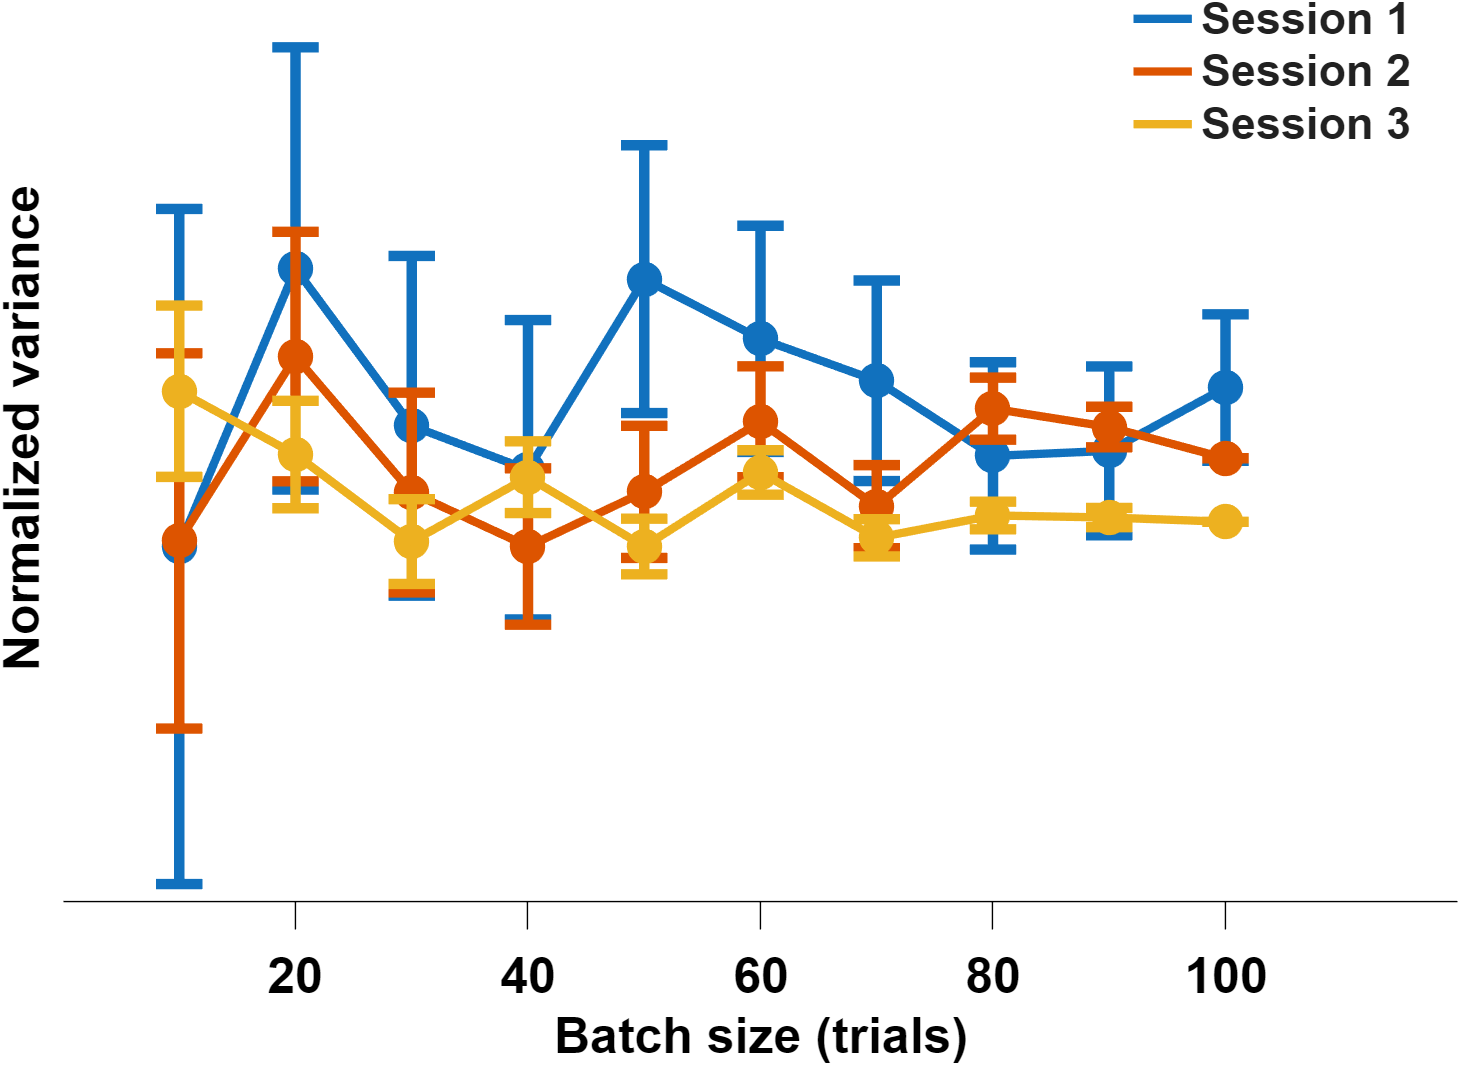
\includegraphics[width=0.5\linewidth]{images/spont_variance.png}
    \caption{Convergence of trial-averaged $\Delta F/F$ variance with batch size, supporting the trial-averaging assumption. Mean total variance $\mathrm{Var}(y_t)$, averaged across the spontaneous-activity window and over five independent random subsamples per batch size, plotted as a function of the number of trials $N$ included in the average. Each line is one session. Variance stabilizes beyond approximately 50 trials per session, indicating that the 100-trial validation blocks provide a reliable estimate of the trial-averaged response.}
    \label{fig:S1}
\end{figure}
%%%%%%%%%%%%%%%%%%%%%%%%%%%%%%%%%%%%%%%%%%%%%%%%%%
\bibliographystyle{apalike}
\bibliography{refs}

\end{document}
